\documentclass[a4paper]{article}
% generated by Docutils <http://docutils.sourceforge.net/>
\usepackage{fixltx2e} % LaTeX patches, \textsubscript
\usepackage{cmap} % fix search and cut-and-paste in Acrobat
\usepackage{ifthen}
\usepackage[T1]{fontenc}
\usepackage[utf8]{inputenc}
\usepackage{graphicx}
\setcounter{secnumdepth}{0}

%%% Custom LaTeX preamble
% PDF Standard Fonts
\usepackage{mathptmx} % Times
\usepackage[scaled=.90]{helvet}
\usepackage{courier}

%%% User specified packages and stylesheets

%%% Fallback definitions for Docutils-specific commands

% hyperlinks:
\ifthenelse{\isundefined{\hypersetup}}{
  \usepackage[colorlinks=true,linkcolor=blue,urlcolor=blue]{hyperref}
  \urlstyle{same} % normal text font (alternatives: tt, rm, sf)
}{}


%%% Body
\begin{document}

% Movie Database with Apex documentation master file, created by
% sphinx-quickstart on Mon Apr 22 16:06:30 2013.
% You can adapt this file completely to your liking, but it should at least
% contain the root `toctree` directive.


\section{Beschreibung und Datenbankschema%
  \label{beschreibung-und-datenbankschema}%
}

Im Rahmen der Studienarbeit Entwicklung von Webanwendungen soll eine Apex
Applikation realisiert werden. Das gewählte Thema umfasst eine Film Metadaten
Plattform, ähnlich dem großem IMDb Vorbild. (www.imdb.com)

Die Film-Datenbank soll die grundlegende Metadaten verwalten können und folgende
Funktionalität bieten:
%
\begin{quote}
%
\begin{itemize}

\item Film Metadaten inklusive Poster-Art + Fan-Art

\item Film Informationen auswertbar nach Genre bzw benutzerdefinierten Tags

\item Informationen zum Regisseur/Drehbuchautor

\item Informationen zu Schauspielern inkl. Foto + Statistiken

\item Verschiedene statistische Auswertungsmöglichkeiten von
Film/Genre/Personen-Metadaten

\item Rating System

\item Erstellen von Favoriten-Listen

\end{itemize}

\end{quote}

Im folgenden ist das Normalisiertes Datenbankschema für die o. g. Applikation:

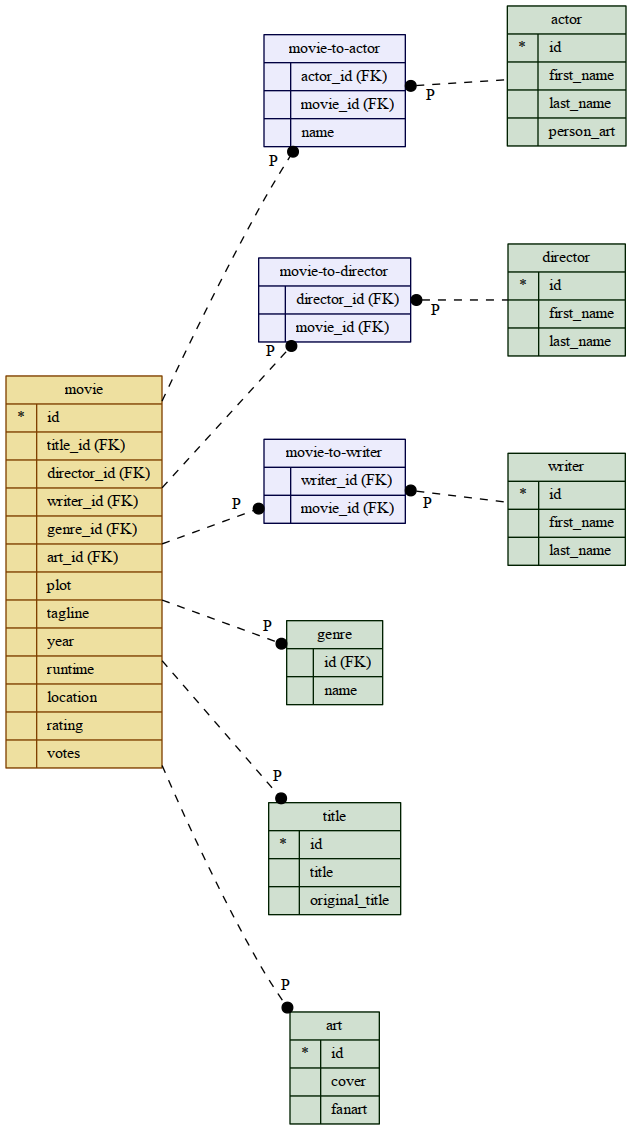
\includegraphics[scale=0.700000]{./dataschema.png}


\section{Main View%
  \label{main-view}%
}

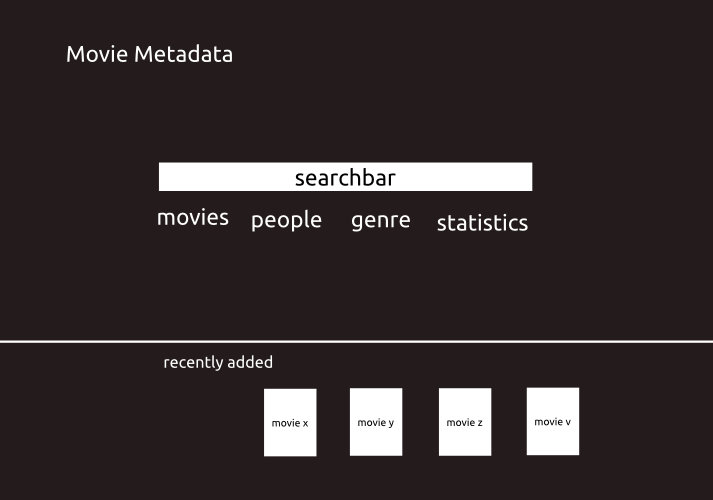
\includegraphics{./mainview.png}

\textbf{Inhalt}:
%
\begin{quote}
%
\begin{itemize}

\item Hauptseite mit Suchfunktion

\item Kürzlich hinzugefügte Filme anzeigen

\item Links zur \textbf{Movies}, \textbf{Genre}, \textbf{Persons} und \textbf{Statistics} Seite

\end{itemize}

\end{quote}


\section{Movie View%
  \label{movie-view}%
}

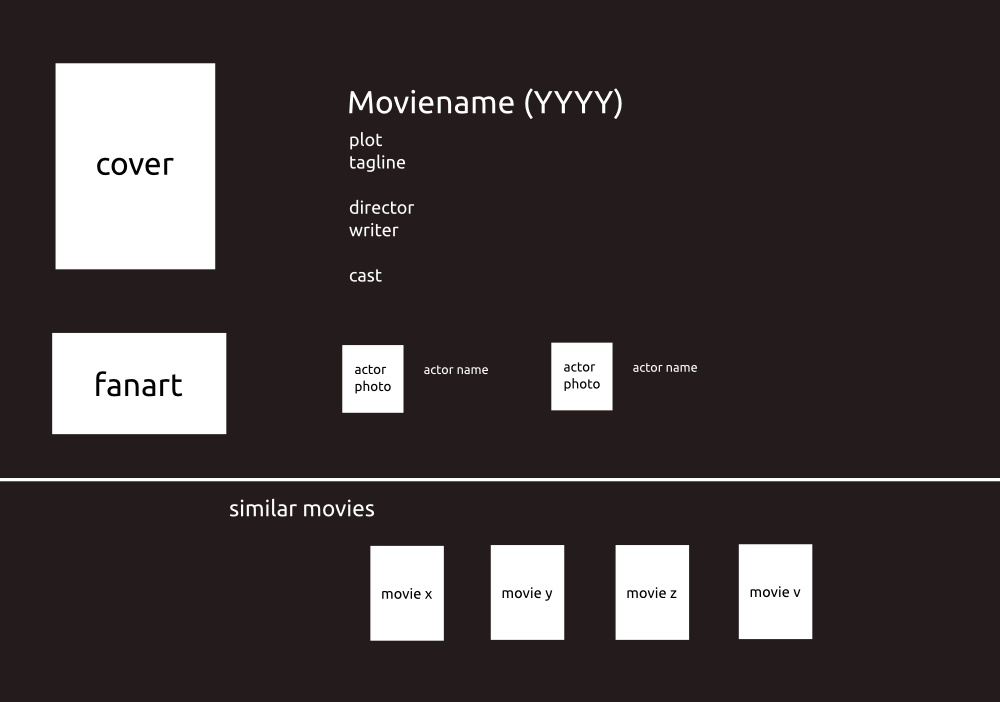
\includegraphics{./movieview.png}

\textbf{Inhalt}:
%
\begin{quote}
%
\begin{itemize}

\item Anzeige von Film-Metadaten, Poster-Art, Fan-Art, Crew und Cast Informationen im
oberen Bereich

\item Anzeige von ,,Similar Movies'' im unteren Bereich

\item Cast/Crew und Similar Movies leiten auf die jeweilige spezialisierte Seite
weiter

\end{itemize}

\end{quote}


\section{Person View%
  \label{person-view}%
}

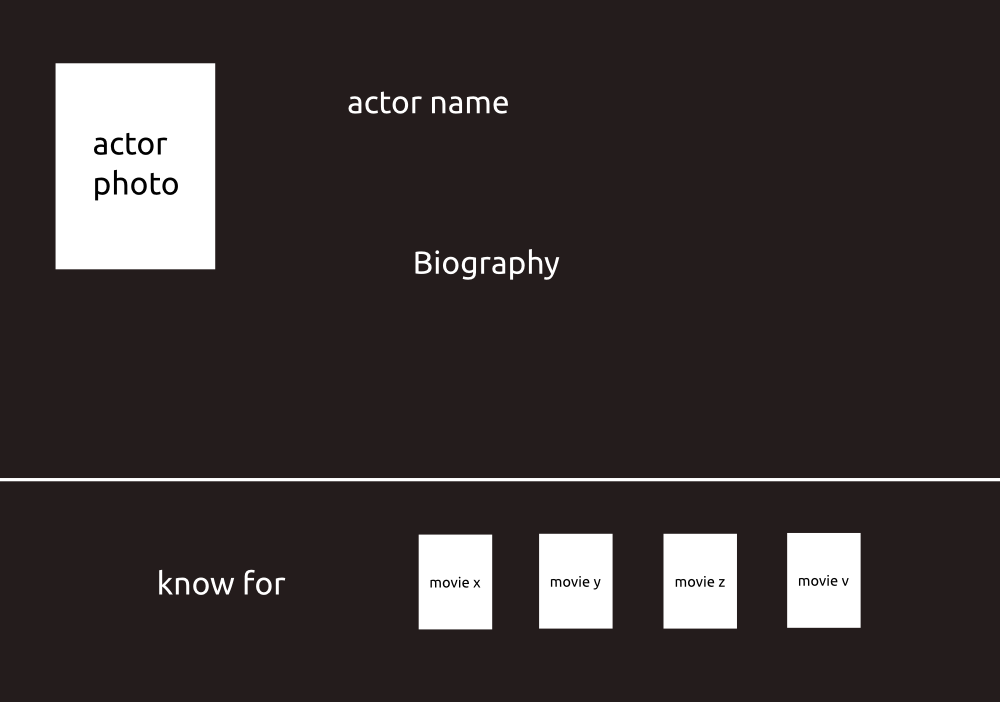
\includegraphics{./actorview.png}
%
\begin{itemize}

\item Anzeigen von Schauspieler-Photo und Biografie im oberen Bereich

\item Anzeigen von Filmen in denen der Schauspieler mitspielt im unteren Bereich

\end{itemize}


\section{Statistics%
  \label{statistics}%
}

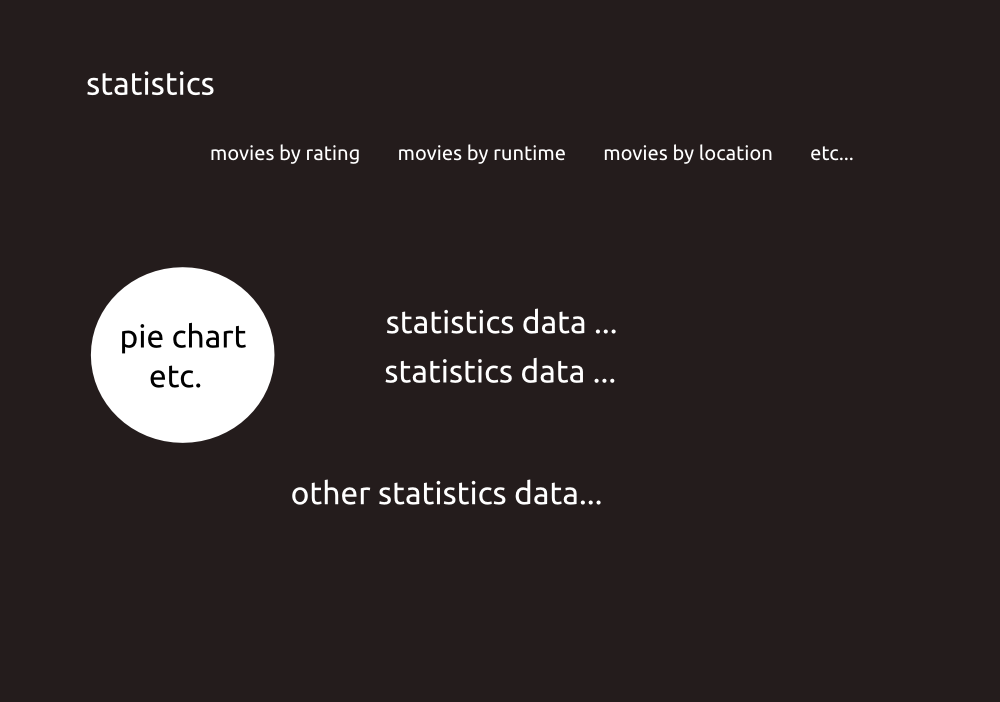
\includegraphics{./statistics.png}

\textbf{Inhalt}:

Anzeige von verschiedenen Statistiken wie z.B.:
%
\begin{quote}
%
\begin{itemize}

\item Liste der besten/schlechtesten Filme

\item Statistische Auswertung nach Laufzeit, Herstellungsland, Rating, etc.

\item Genre Charts (z.B. Tortendiagramm)

\item Person Charts nach Filmgenre

\item Rating Chart

\item Statistiken zu gesehenen und eingetragenen Filmen

\item Favoriten Listen und Statistiken erstellen

\end{itemize}

\end{quote}

\end{document}
